\documentclass[french]{article}
\usepackage[T1]{fontenc}
\usepackage[utf8]{inputenc}
\usepackage{lipsum}
\usepackage{lmodern}
\usepackage{geometry}
\usepackage{babel}
\usepackage{graphicx}
\usepackage{lastpage}
\usepackage{ragged2e}
\usepackage{enumitem}
\usepackage[normalem]{ulem}
\usepackage{hyperref} % pour \url{URL}
\usepackage{color} % pour \textcolor{color}{text}
\usepackage{listings} % pour afficher du code
\usepackage{longtable} % pour l'environnement longtable
\usepackage{float} % pour des figures non flottantes
\usepackage{amsmath}
\usepackage{verbatim} % pour les graphes
\usepackage{caption} % figure et subfigure pour mettre les images côtes à côtes
\usepackage{subcaption}
\usepackage{dirtree}
\usepackage{pdfpages}
% Pdf
\setboolean{@twoside}{false}

% Grammaire EBNF
\usepackage{syntax}
\setlength{\grammarparsep}{5pt plus 1pt minus 1pt}
\setlength{\grammarindent}{11em}

% Dessin avec tikz
\usepackage{tikz}
\usetikzlibrary{shapes,arrows,positioning,shadows,matrix,automata}

% Matrices
\usepackage{kbordermatrix}% http://www.hss.caltech.edu/~kcb/TeX/kbordermatrix.sty

% Largeur de colonnes de tableau fixes
\usepackage{array}
\newcolumntype{L}[1]{>{\raggedright\let\newline\\\arraybackslash\hspace{0pt}}m{#1}}
\newcolumntype{C}[1]{>{\centering\let\newline\\\arraybackslash\hspace{0pt}}m{#1}}
\newcolumntype{R}[1]{>{\raggedleft\let\newline\\\arraybackslash\hspace{0pt}}m{#1}}


% CSS
\lstdefinelanguage{CSS}{
	keywords={color,background-image:,margin,padding,font,weight,display,position,top,left,right,bottom,list,style,border,size,white,space,min,width, transition:, transform:, transition-property, transition-duration, transition-timing-function},	
	sensitive=true,
	morecomment=[l]{//},
	morecomment=[s]{/*}{*/},
	morestring=[b]',
	morestring=[b]",
	alsoletter={:},
	alsodigit={-}
}

% JavaScript
\lstdefinelanguage{JavaScript}{
	morekeywords={typeof, new, true, false, catch, function, return, null, catch, switch, var, if, in, while, do, else, case, break, let},
	morecomment=[s]{/*}{*/},
	morecomment=[l]//,
	morestring=[b]",
	morestring=[b]',
	morestring=[s]{/[}{/;}
}

\lstdefinelanguage{HTML5}{
	language=html,
	sensitive=true,	
	alsoletter={<>=-},	
	morecomment=[s]{<!-}{-->},
	tag=[s],
	otherkeywords={
		% General
		>,
		% Standard tags
		<!DOCTYPE,
		</html, <html, <head, <title, </title, <style, </style, <link, </head, <meta, />,
		% body
		</body, <body,
		% Divs
		</div, <div, </div>, 
		% Paragraphs
		</p, <p, </p>,
		% scripts
		</script, <script,
		% More tags...
		<canvas, /canvas>, <svg, <rect, <animateTransform, </rect>, </svg>, <video, <source, <iframe, </iframe>, </video>, <image, </image>, <header, </header, <article, </article
	},
	ndkeywords={
		% General
		=,
		% HTML attributes
		charset=, src=, id=, width=, height=, style=, type=, rel=, href=,
		% SVG attributes
		fill=, attributeName=, begin=, dur=, from=, to=, poster=, controls=, x=, y=, repeatCount=, xlink:href=,
		% properties
		margin:, padding:, background-image:, border:, top:, left:, position:, width:, height:, margin-top:, margin-bottom:, font-size:, line-height:,
		% CSS3 properties
		transform:, -moz-transform:, -webkit-transform:,
		animation:, -webkit-animation:,
		transition:,  transition-duration:, transition-property:, transition-timing-function:,
	}
}

\lstdefinestyle{htmlcssjs} {%
	% General design
	%  backgroundcolor=\color{editorGray},
	basicstyle={\footnotesize\ttfamily},   
	frame=b,
	% line-numbers
	xleftmargin={0.75cm},
	numbers=left,
	stepnumber=1,
	firstnumber=1,
	numberfirstline=true,	
	% Code design
	identifierstyle=\color{black},
	keywordstyle=\color{blue}\bfseries,
	ndkeywordstyle=\color{black}\bfseries,
	stringstyle=\color{brown}\ttfamily,
	commentstyle=\color{gray}\ttfamily,
	% Code
	language=HTML5,
	alsolanguage=JavaScript,
	alsodigit={.:;},	
	tabsize=2,
	showtabs=false,
	showspaces=false,
	showstringspaces=false,
	extendedchars=true,
	breaklines=true,
	% German umlauts
	literate=%
	{Ö}{{\"O}}1
	{Ä}{{\"A}}1
	{Ü}{{\"U}}1
	{ß}{{\ss}}1
	{ü}{{\"u}}1
	{ä}{{\"a}}1
	{ö}{{\"o}}1
}
%
\lstdefinestyle{py} {%
	language=python,
	literate=%
	*{0}{{{\color{lightred}0}}}1
	{1}{{{\color{lightred}1}}}1
	{2}{{{\color{lightred}2}}}1
	{3}{{{\color{lightred}3}}}1
	{4}{{{\color{lightred}4}}}1
	{5}{{{\color{lightred}5}}}1
	{6}{{{\color{lightred}6}}}1
	{7}{{{\color{lightred}7}}}1
	{8}{{{\color{lightred}8}}}1
	{9}{{{\color{lightred}9}}}1,
	basicstyle=\footnotesize\ttfamily, % Standardschrift
	numbers=left,               % Ort der Zeilennummern
	%numberstyle=\tiny,          % Stil der Zeilennummern
	%stepnumber=2,               % Abstand zwischen den Zeilennummern
	numbersep=5pt,              % Abstand der Nummern zum Text
	tabsize=4,                  % Groesse von Tabs
	extendedchars=true,         %
	breaklines=true,            % Zeilen werden Umgebrochen
	keywordstyle=\color{blue}\bfseries,
	frame=b,
	commentstyle=\color{gray}\itshape,
	stringstyle=\color{brown}\ttfamily, % Farbe der String
	showspaces=false,           % Leerzeichen anzeigen ?
	showtabs=false,             % Tabs anzeigen ?
	xleftmargin=17pt,
	framexleftmargin=17pt,
	framexrightmargin=5pt,
	framexbottommargin=4pt,
	%backgroundcolor=\color{lightgray},
	showstringspaces=false,      % Leerzeichen in Strings anzeigen ?
}%

\geometry{
	a4paper,
	total={210mm,297mm},
	left=20mm,
	right=20mm,
	top=20mm,
	bottom=20mm,
}

\usepackage{fancyhdr}
\pagestyle{fancy}
\setlist[enumerate,1]{leftmargin=2cm}

% Entêtes
\lhead{Champion, Loiseau\\Rochat, Schubert}
\chead{}
\rhead{PDG: Rapport}
\renewcommand{\headrulewidth}{0.4pt}
\renewcommand{\footrulewidth}{0.4pt}

\begin{document}
	
	
	% Titre du document
	\title{Projet Rady} % ou un autre nom\centering
	\author{Rapport\\ 
		Projet de groupe\\
		Champion, Loiseau, Rochat, Schubert\\
		Resp. René Rentsch\\
		HEIG-VD}
	\date{\today} % date du jour
	\maketitle
	\vspace{2cm}
	\centering
	
\includegraphics[scale=0.3]{../logo/icone}
	\thispagestyle{empty}
	
	\newpage
	\thispagestyle{empty}
	$ $
	\newpage
	
	% Pour tout le document
	\justify
	\normalsize
	
	% Tables des matières
	\tableofcontents
	
	\newpage
	
	\section*{Remerciements}
	Nous tenons tout d'abord à remercier M. Prof. René Rentsch pour son suivi et ses conseils durant toute la période du travail. Nous voulons également à remercier M. Prof. Olivier Liechti pour son aide dans le choix des technologies.
	
	\section{Introduction}
	Dans le cadre du cours PDG en troisième année du cursus de Bachelor de la HEIG-VD, il a été demandé de réaliser un projet de semestre sur une période de 10 semaines. Après l'acceptation du cahier des charges à la semaine 4, le projet a pu débuter. Celui-ci porte sur la réalisation d'une application mobile permettant de se retrouver facilement entre amis notamment lors d'évènements. L’application se présenterait sous la forme d’une liste d’amis, laquelle permettrait de créer des groupes et de lancer une rencontre. L’utilisateur aurait alors le choix entre une carte en vue du dessus ou une boussole indiquant la direction à prendre.
	TODO : DECRIRE HIERARCHIE DU RAPPORT
	
		\subsection{Objectif}
		Les objectifs principaux de notre application peuvent être décomposés en trois grandes parties. Premièrement, la gestion des utilisateur, qui comprends la création de compte, la gestion du-dit compte, ainsi que la recherche et l'ajout d'amis. Ensuite, l'intégration de la géolocalisation dans notre application doit permettre, par des appels à une API, aux utilisateurs de se retrouver. Cela constitue la partie centrale de l'application. Enfin, étant donné que des informations sensibles transiteront sur le réseau par le biais de notre application, une attention particulière sera mise vis-à-vis de la sécurité.\\
		Toutes les spécifications précises sont disponibles dans le cahier des charges fourni en annexe.
		
		\subsection{Architecture}
		L’application est composée d’une partie cliente (l'application mobile a proprement parlé), d’un serveur (hébergé sur une machine distante) communiquant avec une base de donnée et faisant appel au service FireBase Cloud Messaging (voir \textbf{figure \ref{Architecture simplifié}}). Le serveur sera à même de gérer la connexion et l’interaction avec plusieurs clients simultanément de manière transparente pour les utilisateurs. \\
		Les données de l’application seront stockées dans une base de données dont l’accès direct se fera uniquement par le serveur. Les clients devront passer par l'API mise à disposition par le serveur pour tout accès aux données, pour des raisons évidentes de sécurité.
		Enfin le serveur fera appel au service FireBase Cloud Messaging (FCM) pour envoyer les notifications de push aux utilisateurs de l'application. 
		
		\begin{figure}[H]
			\centering
			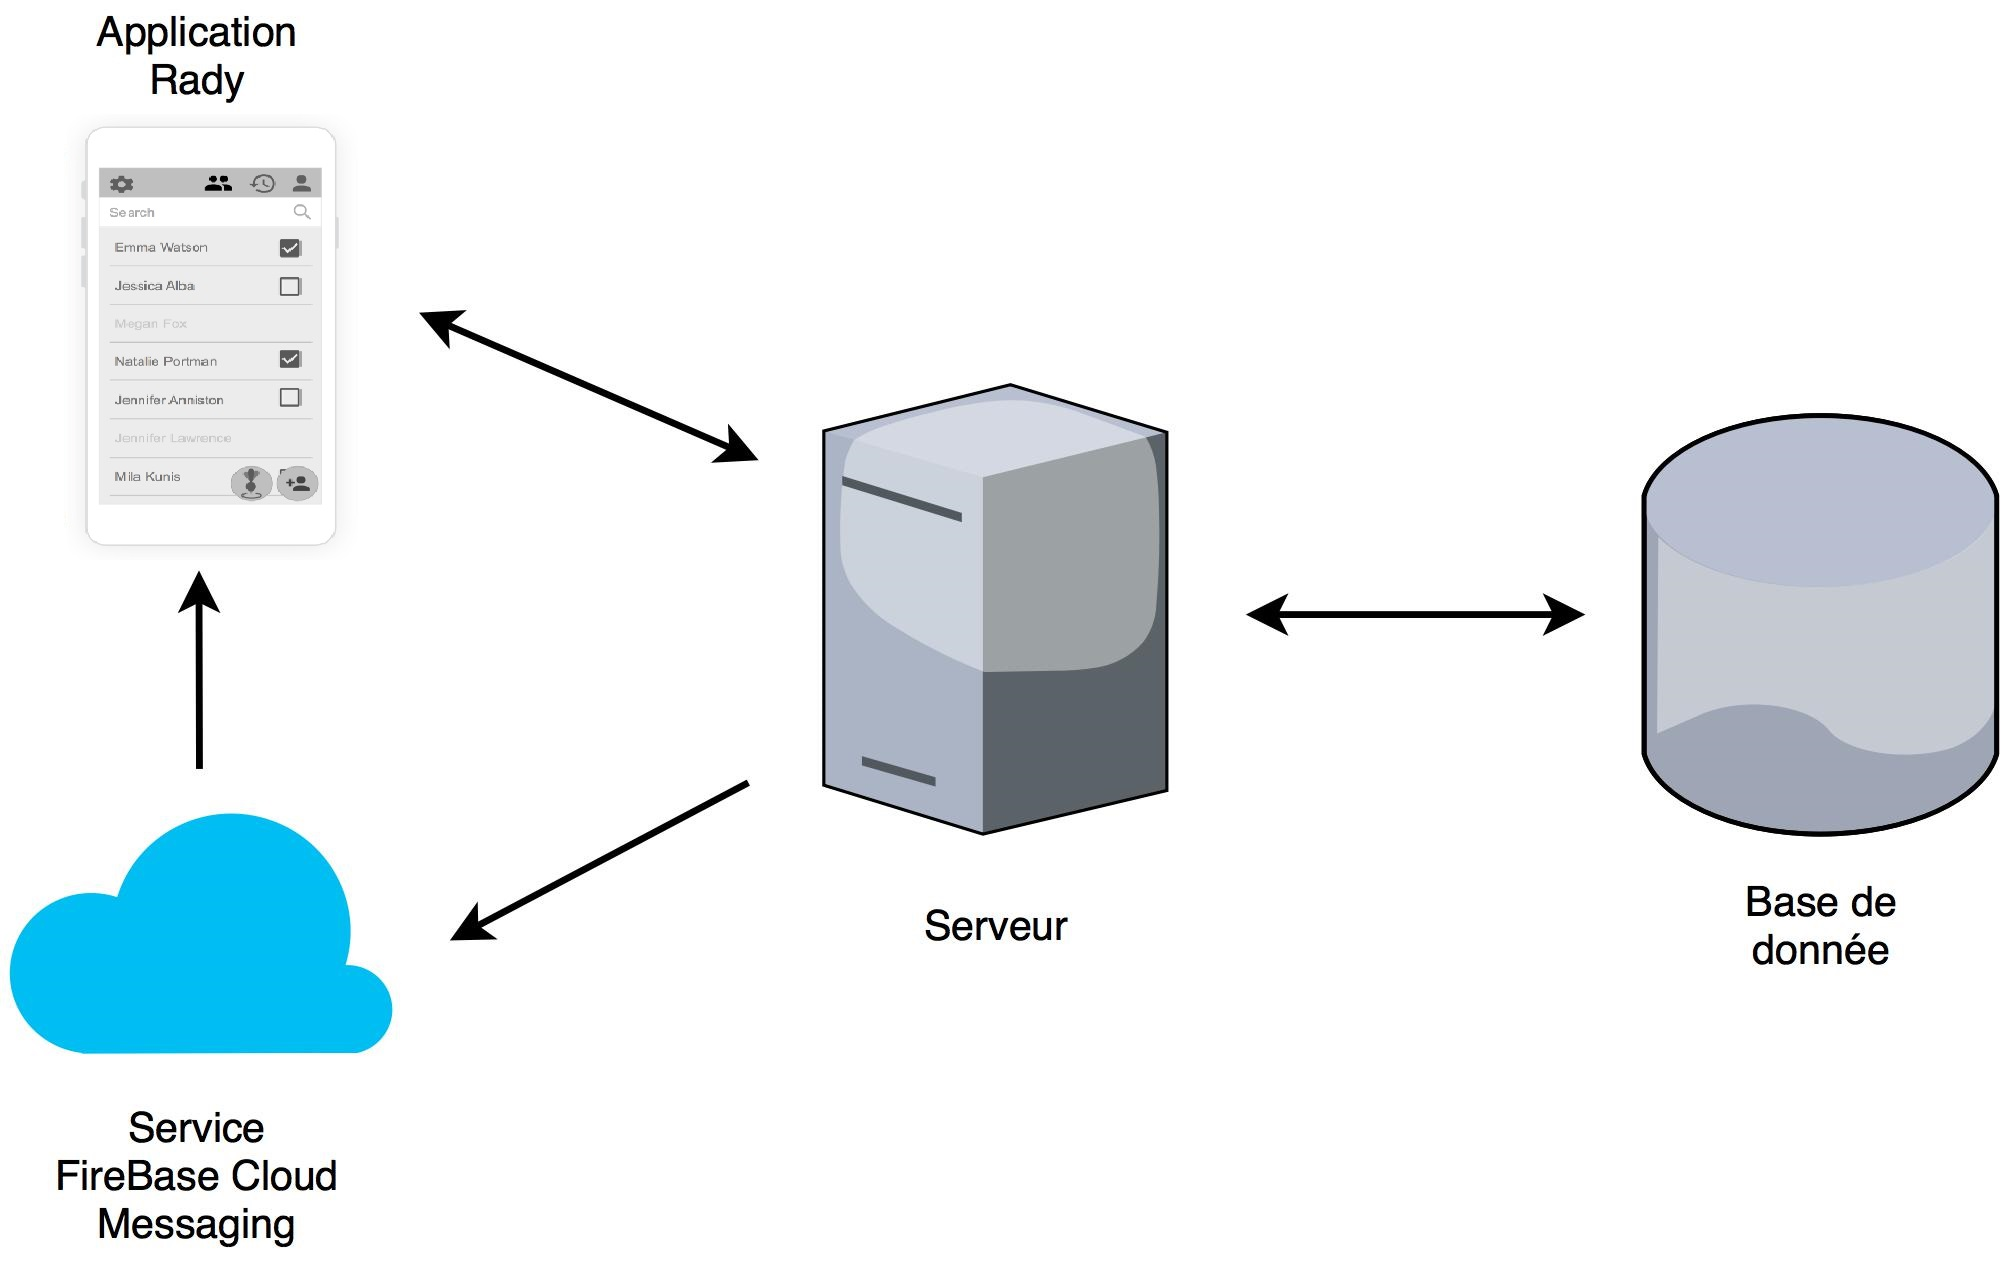
\includegraphics[scale=0.20]{../schema/schema-simplifie.jpg}
			\caption{Architecture simplifiée}
			\label{Architecture simplifié}
		\end{figure}
		
		La conception générale de l'application a été divisée dans ces mêmes différentes parties afin de réduire les dépendances au niveau du développement (temps d'attente sur le travail des autres) ainsi que le nombre de conflit sur le gestionnaire de version (git).
		
		\subsection{Choix des technologies}
		Le choix des technologie a été un point clé lors de l'élaboration du cahier des charges et les premières étapes du développement à proprement parlé du projet.
		Nous avons essayé de choisir les technologies de manière à ce qu'elles soient maintenables et performantes.
		\begin{itemize}
			\item \textbf{Interface :} Pour l'interface nous pensions tout d'abord à utiliser \textbf{MeteorJS} \cite{meteor}, étant donné qu'il s'agit d'un framework pemettant un developpement "cross-plateform" performant. Cependant notre choix s'est finalement porté sur un autre framework "cross-plateform" \textbf{Ionic2} \cite{ionic}, étant donné que \textbf{MeteorJS} est un framework dit "fullstack". Cela signifie qu'on aurait du développer avec ce framework de bout en bout, ce qui aurait pu compromettre le développement en cas de difficulté sur une des parties.
			\item \textbf{Serveur :} Concernant le serveur nous avons choisi d'utiliser \textbf{Django} \cite{django}  pour ses performances, sa sécurité, sa scalabilité et sa maintenabilité.
			\item \textbf{Base de données :} Le choix de la base de données s'est porté sur \textbf{PostgreSQL} car ce système de gestion de base de données (SGBD) est stable, fonctionne sur de nombreux OS et peut stocker des types de données dit "modernes". De plus ce SGDB fait parti des plus conforme aux norme ANSI SQL.
			\item \textbf{Serialisation :} Pour la sérialisation des données et leur transfert nous avons opté pour \textbf{JSON}, car en comparaison avec \textbf{XML}, le \textbf{JSON} est plus léger, plus simple et peut directement être utilisé par le TypeScript (Ionic2), ainsi qu'être stocké tel quel dans le SGBD.
			\item \textbf{Notifications :} Le systeme de notification permettant au serveur de maintenir les utilisateurs à jour concernant les interactions inter-utilisateur se fera via \textbf{Firebase Cloud Messsaging}. FCM  (anciennement Google Cloud Messaging) nous offre un service de transmission de message fiable, une plus grande simplicité de développement ainsi qu'une prise en charge multi-plateforme.
		\end{itemize}
		
		\begin{figure}[H]
			\centering
			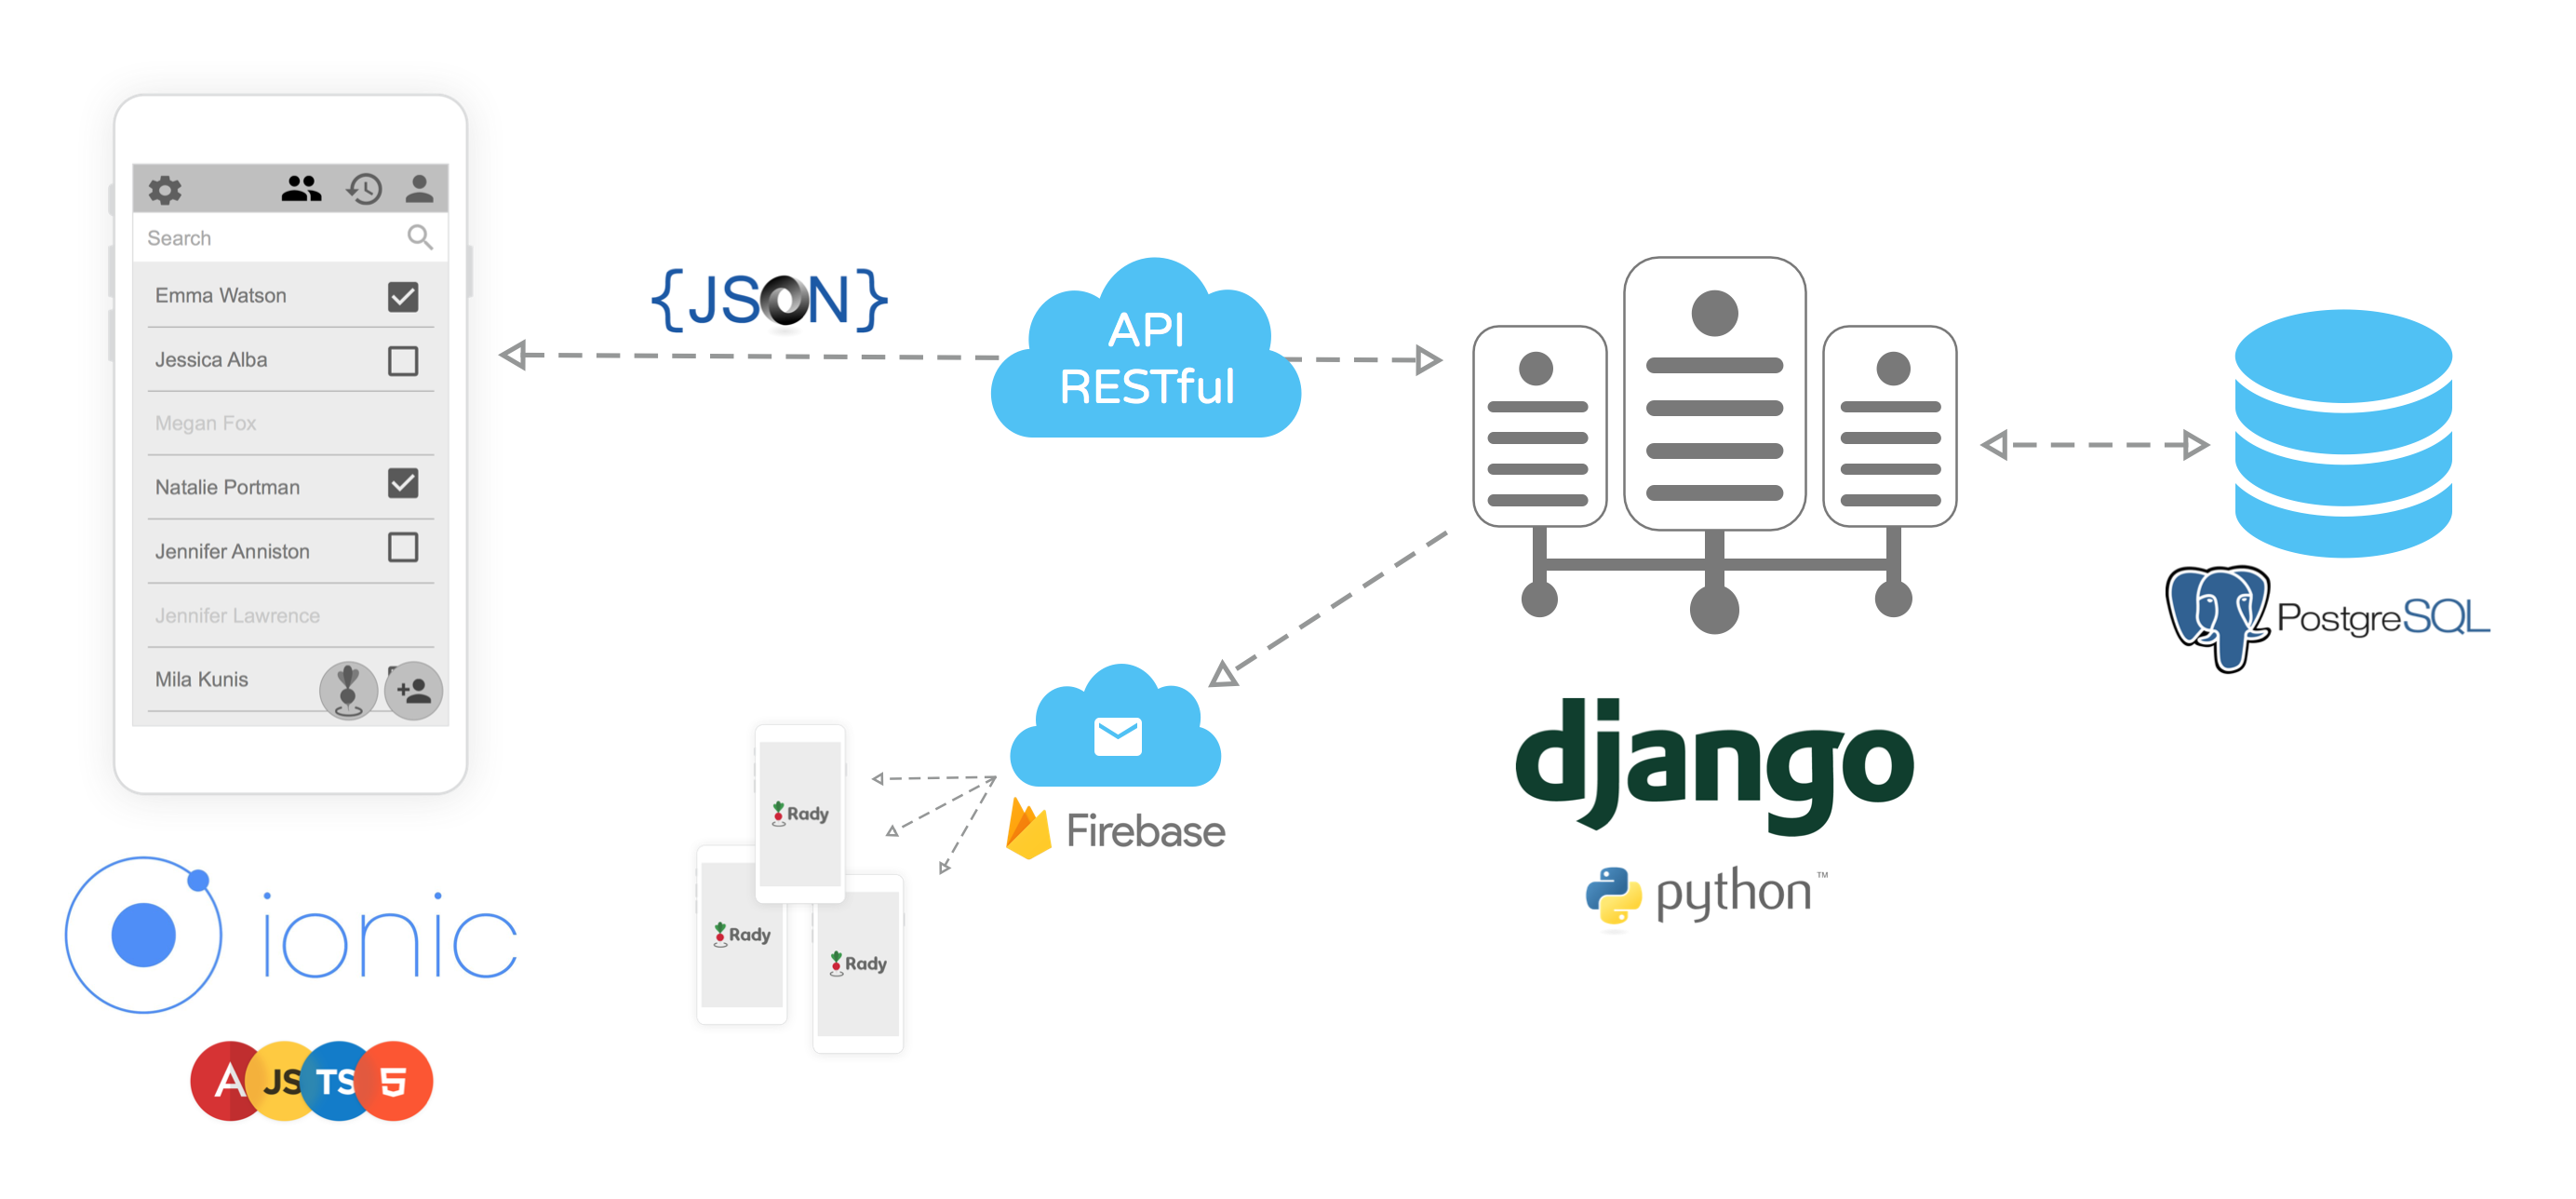
\includegraphics[scale=0.35]{../schema/schema-techno.png}
			\caption{Architecture et Technologies}
			\label{Architecture et Technologies}
		\end{figure}
		
	
	\section{Cadre de développement} 
		Le client de l'application a été développé en TypeScript(2.0.9) et angular2(2.2.1), avec node.js(6.9.1) et le gestionnaire de paquet npm(3.10.9). Le serveur quand à lui a été développé avec python(3.5.2). 
		Nous avons également utilisé un service web d'hébergement et de gestion de développement de logiciels : GitHub, avec le logiciel de gestion de version Git, afin de gérer la mise en commun du code et l'intégration des différentes fonctionnalités au projet.
		Par ailleurs nous avons aussi utilisé un serveur d'intégration continue (Travis) afin de pouvoir vérifier en temps réel le bon déroulement de notre projet.
		Enfin nous avons mis en place des séries de tests visant à faire en sorte que l'API fournie par le serveur soit utilisable et ne contienne pas de faille.
			
	\section{Application Client}
	
	Lors du développement de notre application, la première étape a été de nous familiariser avec les différentes technologies et "frameworks" nécessaire à la réalisation du produit final. Ensuite nous avons décidé de réaliser une maquette de l'interface que l'utilisateur final utilisera. Cette maquette a été conçue pour être simple et permettre une utilisation intuitive de l'application. Enfin il a fallut développer les menus et interfaces de l'application et lier les contrôleurs aux différentes fonctionnalités.
	
	\subsection{Frameworks}
	
	\subsubsection{Ionic2}
	
	\begin{figure}[H]
		\centering
		
\includegraphics[scale=0.45]{../images/ionic2-logo.png}
		\caption{Ionic2 logo}
		\label{Ionic2 logo}
	\end{figure} 
	
	Notre application a été réalisée avec le framework Ionic2. Ce framework, disponible depuis septembre 2016, se distingue de sa version précédente Ionic en incluant la syntaxe ES6, une nouvelle structure de fichier et en intégrant une CLI plus perfectionnée permettant la génération automatique de pages.
	L’interface graphique est décrite par un fichier HTML utilisant des composants spécifiques à Ionic2 :
	
	\lstset{language = HTML5}
	\begin{lstlisting}
	<ion-component>
	\end{lstlisting}
	
	Les balises permettent de placer les différents éléments de l’interface un peu à la manière dont on structure une page en HTML standard. La personnalisation des éléments se fait grâce à des styles CSS, spécifiés soit dans les attributs des éléments, soit via des feuilles de style externes dans les fichiers SCSS. Les attributs du SCSS diffèrent un peu des attributs CSS standards, ils permettent d'utiliser les SASS (Syntactically Awesome Style Sheets). Les fichier SCSS seront utilisés pour régénérer le CSS nécessaire à l'affichage des styles. 
	A chaque fichier HTML et SCSS vient s’ajouter un fichier de code TypeScript, qui sert de contrôleur pour l’interface. Dans le HTML on définit les différents évènements de l’interface (par exemple un clic sur un bouton, ou un changement d'état d'un élément de type bascule) en déclenchant un appel de méthode au niveau du fichier contrôleur (le ficher TypeScript), qui gère ensuite l’évènement. Il est également possible d’ajouter et modifier des balises HTML directement depuis le contrôleur TypeScript afin de rendre l’interface plus dynamique, en la faisant par exemple réagir aux interactions de l’utilisateur ou aux réponses du serveur. 
	
	Voici la structure des sources de l'application mobile :
	
	\begin{figure}[H]
		\centering
		\dirtree{%
			.1 src/\DTcomment{répertoire contenant les sources de l'application}.
			.2 app/\DTcomment{répertoire contenant les liens des différents composants}.
			.3 app.component.ts\DTcomment{fichier définissant la page d'accueil}.
			.3 app.html\DTcomment{permet de lancer la page d'accueil}.
			.3 app.modules.ts\DTcomment{permet de charger les différents modules et interfaces}.
			.3 app.scss\DTcomment{styles portant sur toute l'application}.
			.3 main.ts\DTcomment{fichier permettant le lancement de l'application}.
			.2 assets/\DTcomment{répertoire contenant les éléments utiles}.
			.2 lib/\DTcomment{répertoire contenant les librairies utilisées}.
			.2 models/\DTcomment{répertoire contenant les modèles(classes) utilisés}.
			.2 pages/\DTcomment{répertoire contenant les différentes interfaces}.
			.3 add-contact/\DTcomment{répertoire contenant les éléments pour l'interface d'ajout de contact}.
			.4 add-contact.html/\DTcomment{code HTML définissant les composants de l'interface}.
			.4 add-contact.scss/\DTcomment{styles s'appliquant aux composants HTML}.
			.4 add-contact.ts/\DTcomment{logique appelés par les composants HTML}.
			.3 contact-list/\DTcomment{répertoire contenant les éléments pour l'interface de gestion de contacts}.
			.4 contact-list.html/\DTcomment{code HTML définissant les composants de l'interface}.
			.4 contact-list.scss/\DTcomment{styles s'appliquant aux composants HTML}.
			.4 contact-list.ts/\DTcomment{logique appelée par les composants html}.
			.3 <...>\DTcomment{autres fichiers d'implémentation}.
			.2 providers/\DTcomment{répertoire contenant les services utilisés par l'application}.
			.2 theme/\DTcomment{répertoire contenant les fichiers .scss appliqués sur toute l'application}.
			.2 declarations.d.ts\DTcomment{fichier de déclaration pour le compilateur TypeScript}.
			.2 index.html\DTcomment{première page chargée par ionic permettant le chargement du reste de l'application}.
			.2 manifest.json\DTcomment{données pour l'affichage de l'application}.
			.2 service-workers.js\DTcomment{fichier contenant un script qui tournera en tâche de fond}.	
		}
	\end{figure}
	
	On observe que les interfaces sont dans le dossier pages avec leurs fichiers HTML, SCSS, et TS correspondants. Dans le dossier app/ on retrouve le lien entre les différentes pages et l'application en elle-même. Ionic2 propose une hiérarchie intuitive regroupant les éléments par nature puis par fonctionnalité (librairies, models ...) afin de simplifier le développement.
	
	\subsubsection{Angular2}
	
	\begin{figure}[H]
		\centering
		
\includegraphics[scale=0.4]{../images/angular2-logo.png}
		\caption{Angular2 logo}
		\label{Angular2 logo}
	\end{figure} 
	
	Angular2 est un framework JavaScript conçu pour simplifier le développement d'interfaces web. Ionic2 nous permet d'utiliser la version 2 de ce framework elle aussi sortie en septembre 2016. 
	Angular2 nous offre la possibilité de réaliser du "data binding" bidirectionnel. C'est-à-dire que lorsque les données affichées dans la vue sont modifiées cela affecte directement le contrôleur qui s'est mis à jour. Ce framework nous donne aussi accès à des directives rendant le code plus extensible et modulable, et nous permet d'utiliser l'injection de dépendance pour l'appel à des services initialisés ailleurs dans le code. 
	
	\subsubsection{Cordova}
	
	\begin{figure}[H]
		\centering
		
\includegraphics[scale=0.4]{../images/cordova-logo.png}
		\caption{Leaflet logo}
		\label{Leaflet logo}
	\end{figure} 
	
	Apache Cordova est un framework open-source qui permet de créer des applications pour différentes plateformes (Android, Firefox OS, iOS, Ubuntu, Windows 8...) en HTML, CSS et JavaScript. C'est lui qui sera appelé par Ionic pour "build" et déployer l'application directement sur le matériel.
	Ce framework permet d'avoir accès aux différentes fonctionnalités et éléments du téléphone tel que la boussole, l'accéléromètre, la géolocalisation ou encore l'appareil photo.
	
	\subsubsection{Leaflet}
	
	Leaflet est une librairie open-source JavaScript pour le développement d'application web de cartographie.
	
	\begin{figure}[H]
		\centering
		
\includegraphics[scale=0.4]{../images/leaflet-logo.png}
		\caption{Leaflet logo}
		\label{Leaflet logo}
	\end{figure} 
	
	
	Cette librairie nous permet non seulement d'afficher une carte, mais aussi des marqueurs que nous utilisons pour afficher les positions des utilisateurs, ainsi que les lieux que nous souhaitons localiser. De plus celle-ci est extrêmement configurable, on peut en effet choisir d'utiliser nos propres éléments à afficher tel que des marqueurs personnalisés ou encore utiliser divers générateurs de carte tel que mapbox, openstreetmap ou encore google map.
	
	\begin{figure}[H]
		\centering
		
\includegraphics[scale=0.4]{../images/mapbox-logo.png}
		\caption{Mapbox logo}
		\label{Mapbox logo}
	\end{figure} 
	
	\subsection{Design}
	
	Il a tout d'abord fallu établir le design de l'application comprenant les différentes interfaces à afficher, l'ordre d'affichage des ces interfaces ainsi que les animations et écrans de chargement à afficher. Ainsi nous avons commencé le projet en établissant un flux d'utilisation:
	
	\begin{figure}[H]
		\centering
		\includegraphics[scale=0.6]{../user-flow/user-flow-1.png}
		\caption{User flow - Loading}
		\label{User flow - Loading}
	\end{figure}
	
	\begin{figure}[H]
		\centering
		\includegraphics[scale=0.6]{../user-flow/user-flow-2.png}
		\caption{User flow - Sign in}
		\label{User flow - Sign in}
	\end{figure}
	
	\begin{figure}[H]
		\centering
		\includegraphics[scale=0.55]{../user-flow/user-flow-3.png}
		\caption{User flow - Main app}
		\label{User flow - Main app}
	\end{figure}
	
	\begin{figure}[H]
		\centering
		\includegraphics[scale=0.55]{../user-flow/user-flow-4.png}
		\caption{User flow - New Contact}
		\label{User flow - New Contact}
	\end{figure}
	
	\begin{figure}[H]
		\centering
		\includegraphics[scale=0.6]{../user-flow/user-flow-5.png}
		\caption{User flow - Gathering}
		\label{User flow - Gathering}
	\end{figure}
	
	
	\subsection{Développement de l'interface}
	\subsubsection{Création des pages}
	
	Le développement des différentes pages a été réalisé en parallèle en répartissant les différents écrans constituant les interfaces finales de notre application.
	La construction des interfaces des menus constituaient la partie la plus simple du développement car ils ne font appel que à des composants simples définis par Ionic2 et seulement quelques directives Angular2. 
	Nous nous sommes efforcés de réaliser des pages les plus proches possible du design réalisé précédemment afin de garder une simplicité de l'interface tant au niveau du développement que au niveau de l'utilisation finale. 
	
	\begin{figure}[H]
		\begin{minipage}[c]{.46\linewidth}
			\centering
			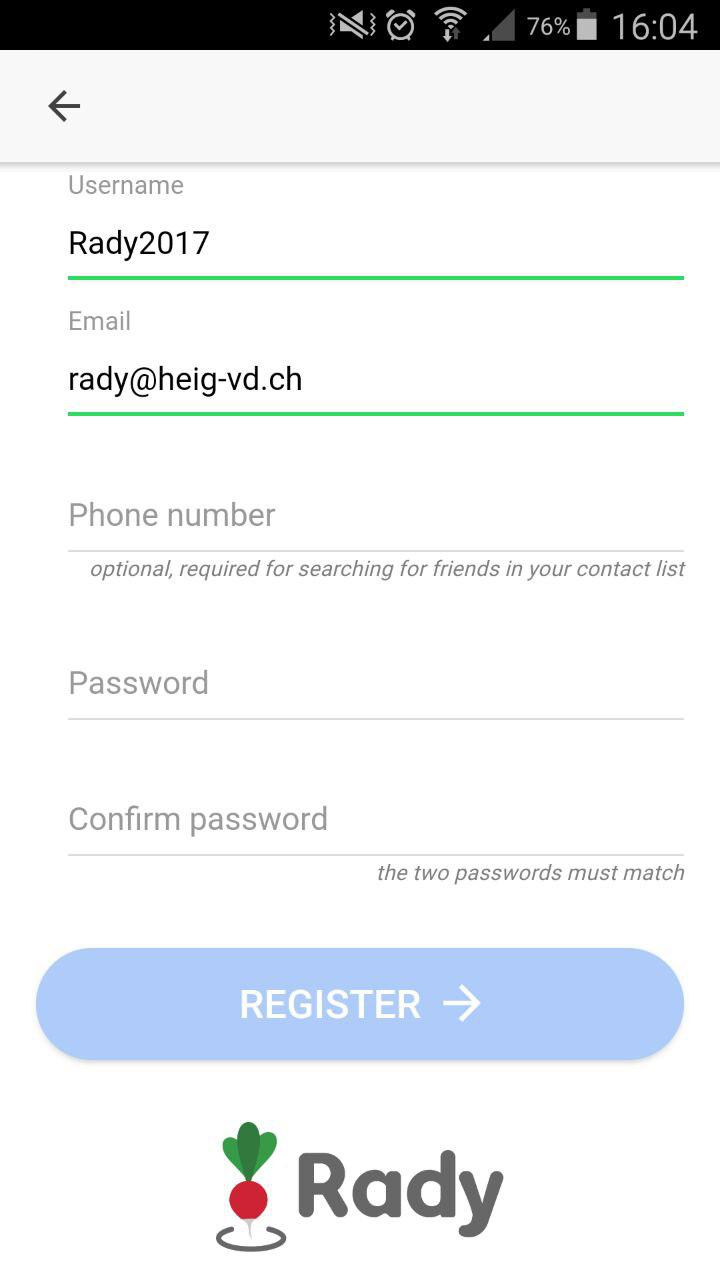
\includegraphics[scale=0.20]{../screenshot/screenshot-register.jpg}
			\caption{Capture d'écran - Enregistrement}
			\label{Capture d'écran - Enregistrement}
		\end{minipage} \hfill
		\begin{minipage}[c]{.46\linewidth}
			\centering
			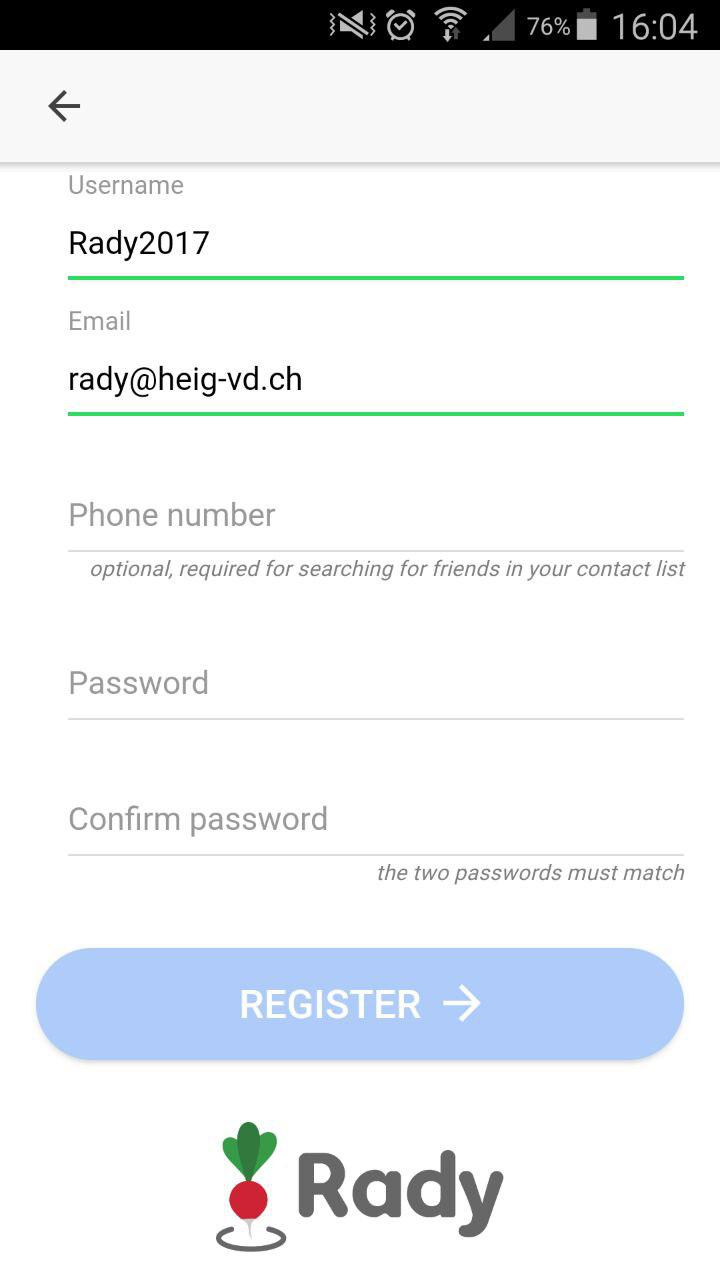
\includegraphics[scale=0.20]{../screenshot/screenshot-register.jpg}
			\caption{Capture d'écran - Test}
			\label{Capture d'écran - Test}
		\end{minipage}
		
	\end{figure} 	 
	
	\newpage
	
	Ensuite est venu l'implémentation des différentes fonctions appelées par les éléments graphiques (vérification des champs, communication avec le serveur, changement de page). Pour ce faire nous avons du créer et utiliser différentes librairies et validateurs.
	
	\subsubsection{Validateurs}
	
	Pour éviter d'effectuer des appels serveur inutile nous avons choisi de faire des tests sur la forme des saisies utilisateur directement dans l'application avant de les envoyer au serveur via l'API afin de diminuer le nombre de réponses négatives. Pour effectuer ces tests nous avons donc eu besoin d'une librairie de validateurs pour nous permettre de définir si la saisie possède la bonne forme ou non. 
	Étant donné que nous n'avons pas trouvé de validateurs correspondant à nos attentes nous avons décidé de les implémenter à la main.
	
	\begin{lstlisting}[style=htmlcssjs]
	/**
	* Email validator
	* Check if the control is a valid email
	* @param emailcontrol
	* @param msg
	*/
	public static email(emailcontrol: string, msg: string) {
		return (group: FormGroup): ValidatorResult => {
			if(group.get(emailcontrol).value.length === 0)
				return null;
			let errors = {};
			let regExp = /[a-z0-9!#$%&'*+/=?^_`{|}~-]+(?:\.[a-z0-9!#$%&'*+/=?^_`{|}~-]+)*@(?:[a-z0-9](?:[a-z0-9-]*[a-z0-9])?\.)+[a-z0-9](?:[a-z0-9-]*[a-z0-9])?/;
			if(!regExp.test(group.get(emailcontrol).value))
			errors[emailcontrol] = msg;
			return Object.keys(errors).length === 0 ? null : errors;
		}
	}
	\end{lstlisting}
	
	Dans ce validateur pour les e-mail nous utilisons une expression régulière, afin de déterminer si l'e-mail entré par l'utilisateur possède une forme correcte. Lorsque le validateur détecte que l'email n'est pas valide, il renvoie une erreur à l'utilisateur qui est instantanément averti.
	Nous utilisons aussi un validateur personnalisé pour les numéros de téléphone afin de déterminer si le numéro est valide suivant l'indicatif du pays. 
	\begin{lstlisting}[style=htmlcssjs]
	/**
	* Phone validator
	* Check if the control the a valid phone
	* @param phonecontrol
	* @param countrycontrol
	* @param msg
	*/
	public static phone(phonecontrol: string, countrycontrol: string, msg: string) {
		return (group: FormGroup): ValidatorResult => {
			if(group.get(phonecontrol).value.length === 0)
				return null;
			let errors = {};
			try {
				const phoneUtil = libphonenumber.PhoneNumberUtil.getInstance();
				const phoneNumber = phoneUtil.parse(group.get(phonecontrol).value, group.get(countrycontrol).value);
				if(!phoneUtil.isValidNumber(phoneNumber))
					errors[phonecontrol] = msg;
				} catch(e) {
					errors[phonecontrol] = msg;
			}
			return Object.keys(errors).length === 0 ? null : errors;
		}
	}
	\end{lstlisting}
	
	Cette fois-ci nous n'utilisons pas d'expression régulière mais nous faisons appel à une librairie externe : libphonenumber.
	Cette librairie permet de passer le numéro de téléphone sous forme canonique, avant de vérifier la cohérence de celui-ci ce qui nous permet de garantir une uniformité de la nature des numéros de téléphone d'un utilisateur à un autre.
	
	 
	
	\subsubsection{Rencontres}
	
	TODO : EXPLICATION + CODE
	
	\subsubsection{Géolocalisation et boussole}
	
	TODO : FONCTIONNEMENT GEOLOC + BOUSSOLE
	TODO : SUCE PAS TROP LA BATTERIE CAR TOUTE LES 3 SECONDES
	
	
	\section{Serveur et Communication}	
	\subsection{Fonctionnement Général}
	
	Afin d'établir le lien entre la partie serveur et la partie cliente, nous avons défini un protocole de communication qui s'occupe de gérer tous les échanges. Celui-ci définit les différents échanges effectués par les applications clientes et le serveur (autant les demandes de ressources que les transmissions de réponse), mais assure également le service de notification de FireBase Cloud Messaging. 
	
	\medbreak
	
	Dans ce protocole nous avons définit que les clients ne communiqueraient jamais directement entre eux ni directement avec la base de donnée ou le service de notification. Toutes leurs requêtes doivent passer par le serveur avec lequel ils communiquent via une API REST. Celui-ci s'occupe de traiter avec la base de données et FireBase Cloud Messaging de manière complètement transparente pour l'utilisateur.
	
	\begin{figure}[H]
		\centering
		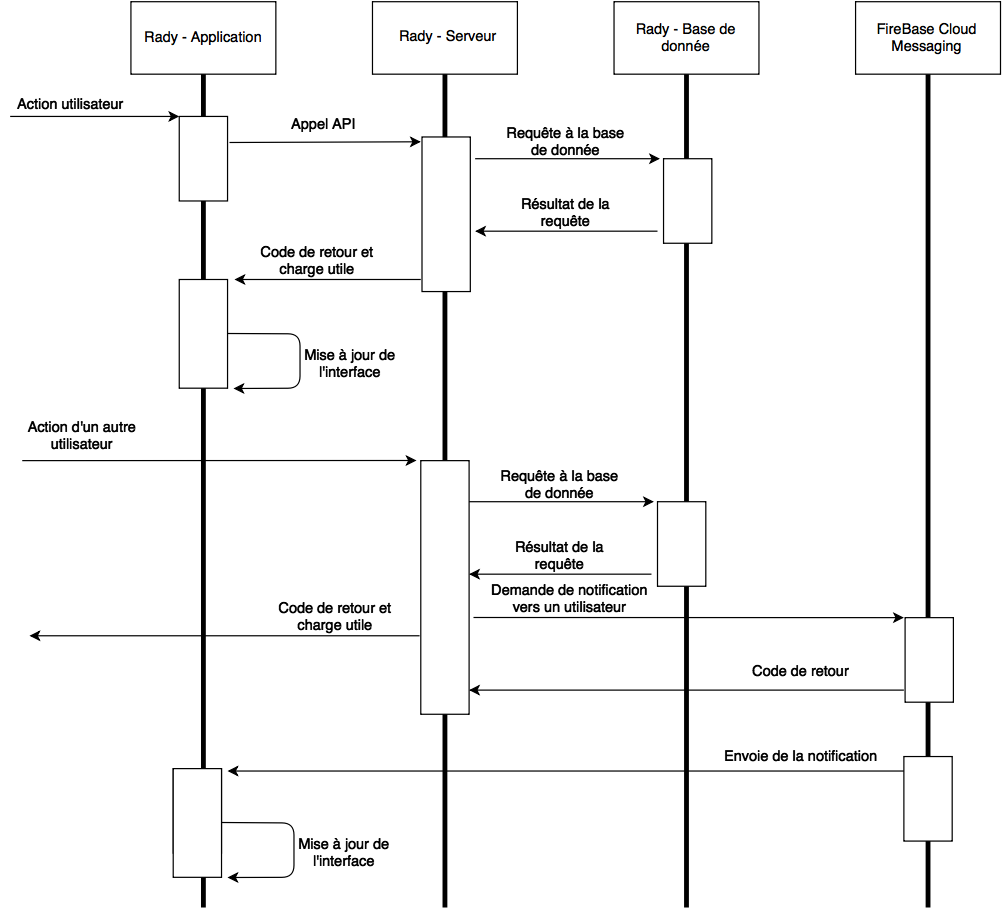
\includegraphics[scale=0.5]{../schema/schema-sequence-communication.png}
		\caption{Diagramme de séquence communication}
		\label{Diagramme de séquence communication}
	\end{figure}
	
	\newpage
	
	\subsection{Base de donnée}	
	Au lancement du serveur, celui-ci fait appel aux services de Django pour créer et déployer la base de données. Un script permet de lancer le serveur et donne des instructions au framework depuis la ligne de commande afin de trouver les différents modèles nécessaires à l'instanciation des tables.
	Django nous permet également de nous rendre complètement indépendant du moteur de base de données que nous souhaitons utiliser.
	Grâce à l'utilisation de Fabric \cite{fabric}, le déploiement est entièrement automatisé.
	\subsubsection{Modèles}
	
	Les entités représentées par les modèles définissent la structure de notre base de données, mais sont aussi le coeur de notre application. 
	En effet, celles-ci constituent les éléments sérialisables échangés à travers le réseau. 
	Ces différents modèles sont définis à la fois en python du coté du serveur ainsi que dans le code TypeScript de l'application Ionic2. Cela permet à notre application de communiquer via un "dialecte" commun avec le serveur malgré une différence de langage de programmation.

	\begin{figure}[H]
		\centering
		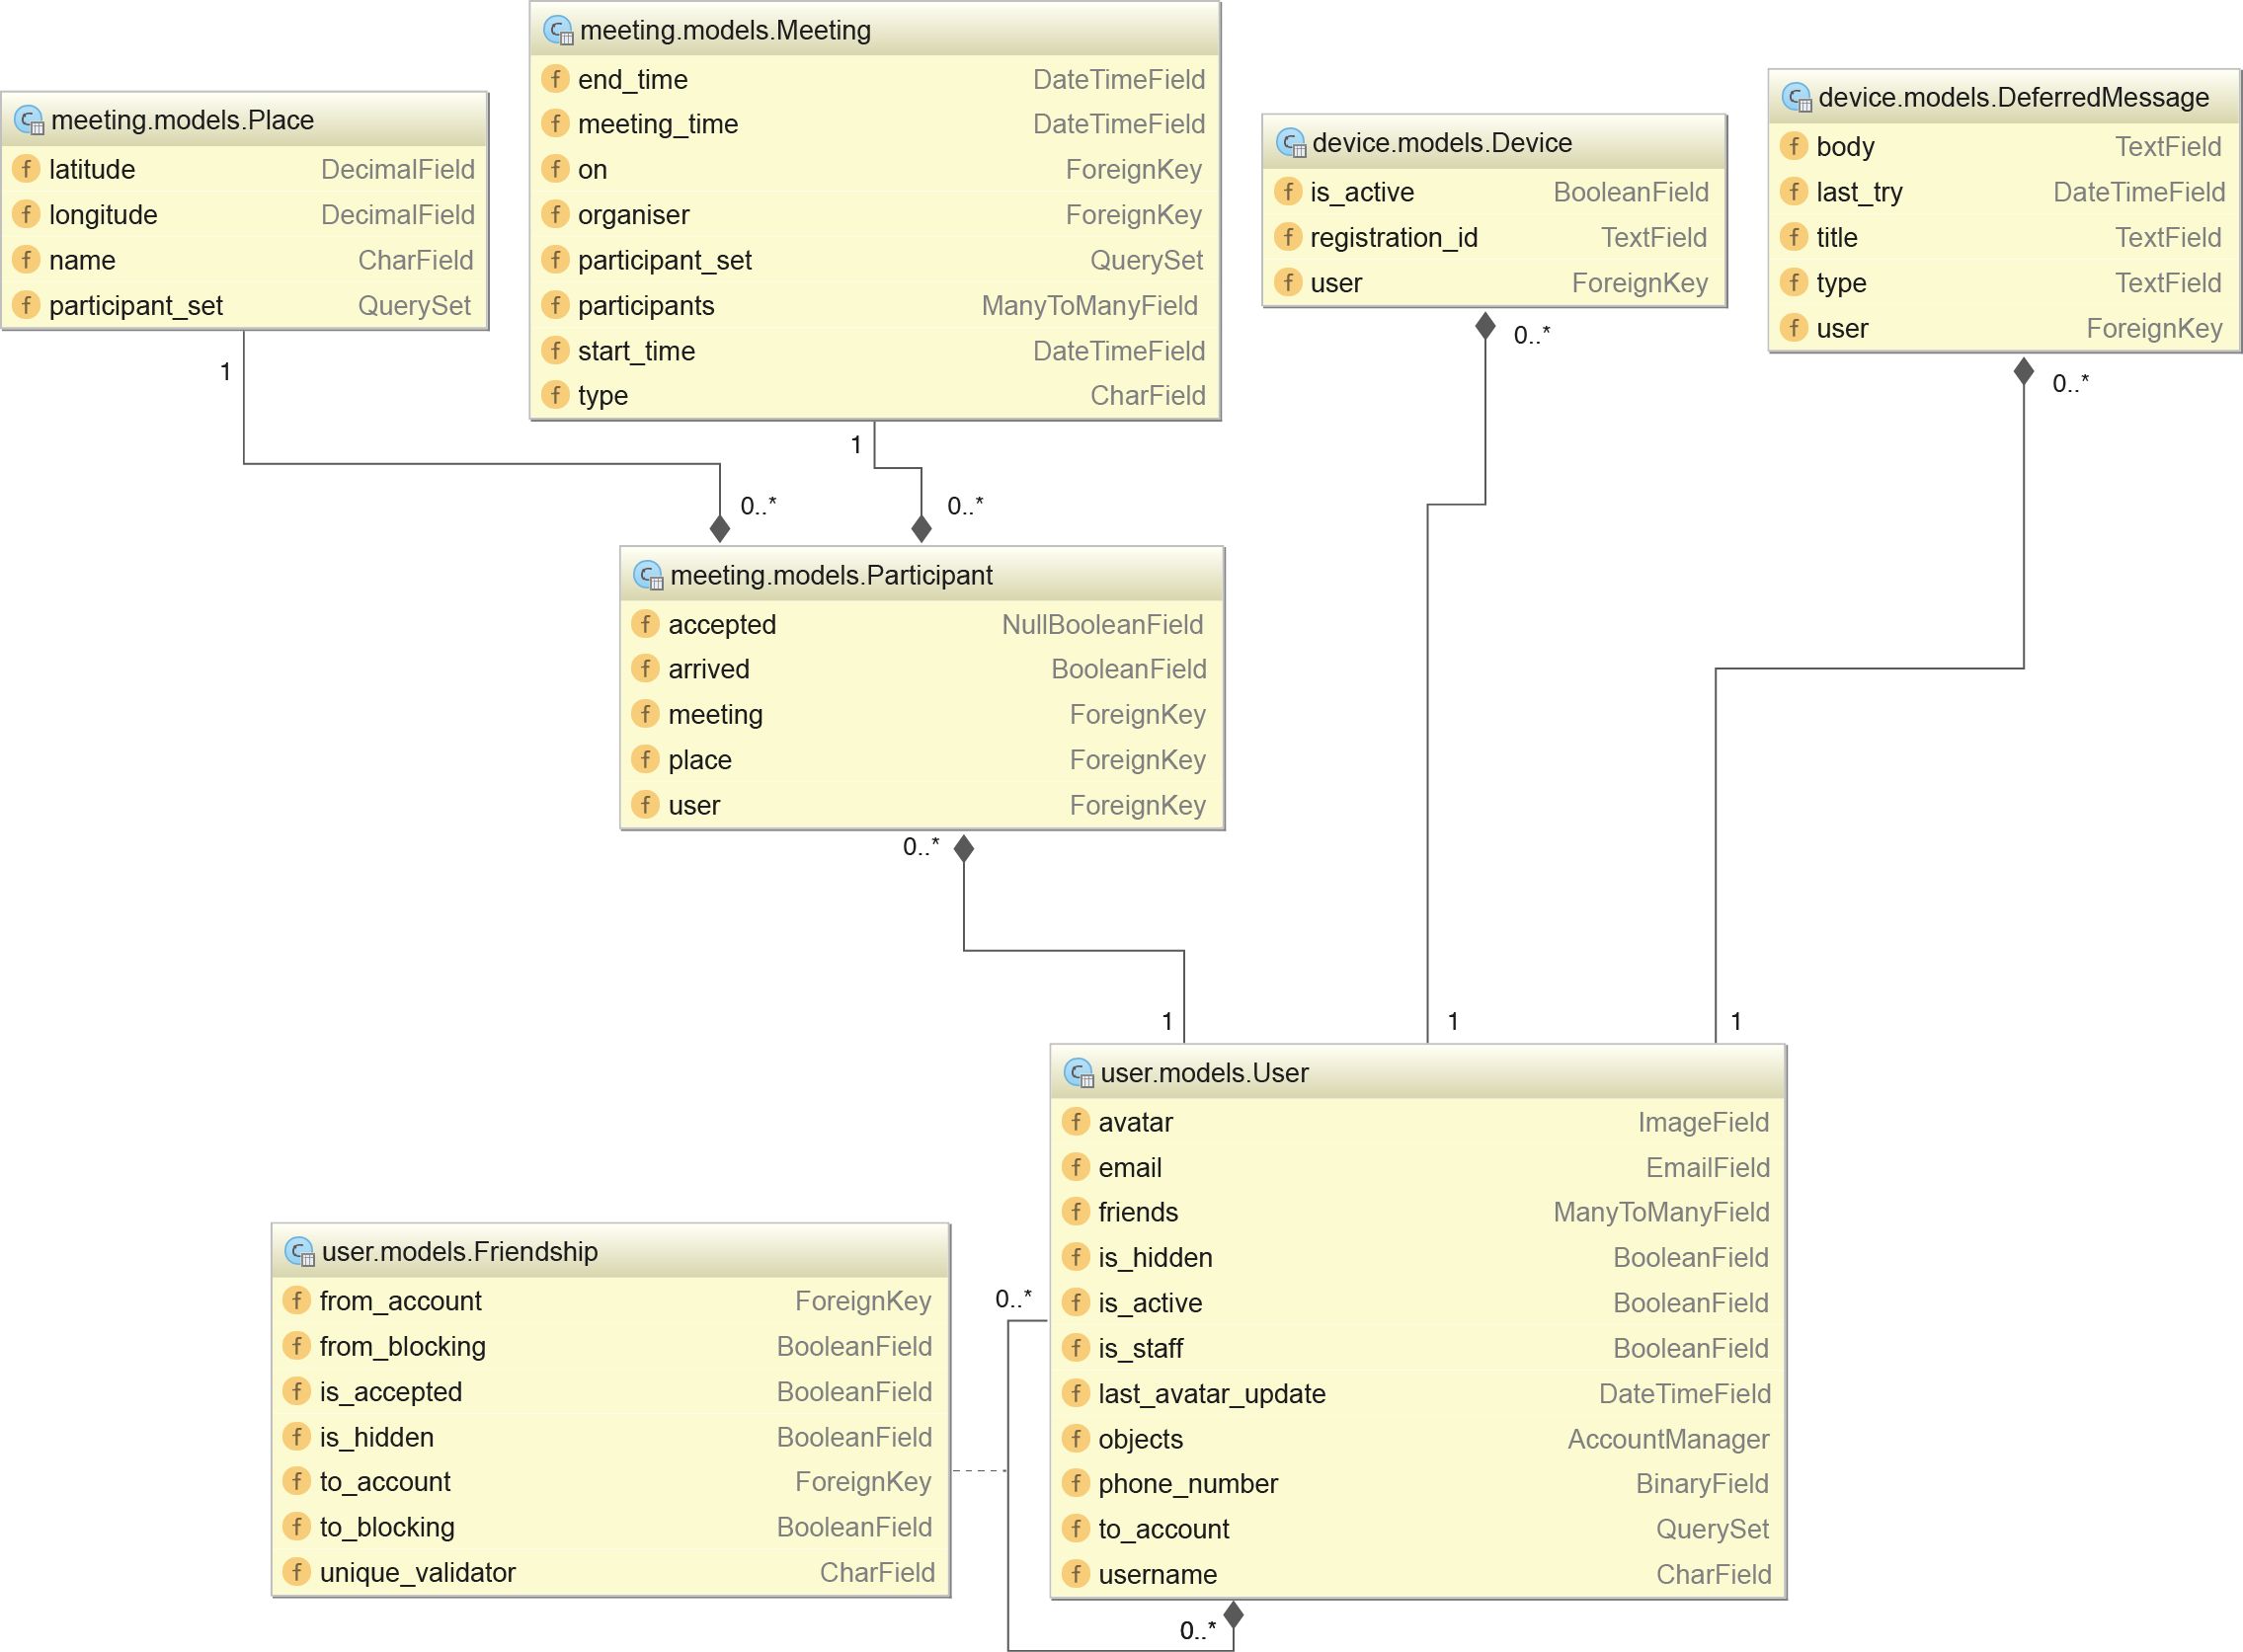
\includegraphics[scale=0.45]{../schema/modele-domaine.png}
		\caption{Modele de domaine}
		\label{Modele de domaine}
	\end{figure}
	
	\subsubsection{Création avec Django}	
	
	Tout d'abord il faut charger les service de Django puis lui demander d'effectuer la création des tables depuis les modèles. Cela s'opère via une ligne de commande lue et transmise à Django dans le fichier : manage.py
	
	\begin{lstlisting}[style=py]
	if __name__ == "__main__":
		os.environ.setdefault("DJANGO_SETTINGS_MODULE", "rady.settings.debug")
		try:
			from django.core.management import execute_from_command_line
		except ImportError:
		# The above import may fail for some other reason. Ensure that the
		# issue is really that Django is missing to avoid masking other
		# exceptions on Python 2.
		try:
			import django # noqa
		except ImportError:
		raise ImportError(
			"Couldn't import Django. Are you sure it's installed and "
			"available on your PYTHONPATH environment variable? Did you "
			"forget to activate a virtual environment?"
		)
		raise
	execute_from_command_line(sys.argv)	
	\end{lstlisting}
	
	Les paramètres entrés en ligne de commande indiquent à Django les opérations à effectuer, c'est à dire la création des différentes tables depuis les modèles pré-existants.
	
	
	
	
	 
	TODO : EXPLICATION DU FONCTIONNEMENT DE DJANGO AVEC POSTGRESQL
	
	
	
	indépendant du moteur de bbd / django
	
	
	\subsection{API}
	
	L'API mise à disposition des usagers est une API REST. Cela signifie que le service fourni possède une interface uniforme, c'est à dire que chaque ressource est identifiée unitairement, que la manipulation de ces ressources se fait via des représentations et que les messages auto-descriptifs expliquent leur nature. De plus cette API met à disposition un implémentation des méthodes du CRUD pour les différents endpoints : 
	\begin{itemize}
		\item[$\bullet$] /users/
		\item[$\bullet$] /users/me/
		\item[$\bullet$] /users/me/avatar/
		\item[$\bullet$] /users/friends/
		\item[$\bullet$] /users/friends/all/
		\item[$\bullet$] /users/friends/blocked/
		\item[$\bullet$] /users/friends/hidden/
		\item[$\bullet$] /users/friends/pending/
		\item[$\bullet$] /users/friends/<pk>/
		\item[$\bullet$] /meetings/
		\item[$\bullet$] /meetings/<pk>/
		\item[$\bullet$] /meetings/places/
		\item[$\bullet$] /meetings/places/<pk>/
		\item[$\bullet$] /meetings/<pk>/participants/
		\item[$\bullet$] /meetings/positions/
		\item[$\bullet$] /auth/login/
		\item[$\bullet$] /auth/refresh/
		\item[$\bullet$] /fcm/devices/
		\item[$\bullet$] /statistics/
		\item[$\bullet$] /admin/users/
		\item[$\bullet$] /admin/users/<pk>/
	\end{itemize}
		
	Nous pouvons observer que ces différents endpoints correspondent directement à des modèles (user, meetings, etc.) ou à des attributs des modèles (avatar, hidden, etc.) qui sont renvoyés ou reçus par l'API. 
	
	\subsection{Notifications}
	\subsubsection{Fonctionnement}
	
	Le système de messages Push, à l'inverse des appels HTTP où le client demande une information au serveur qui lui répond, permet à ce dernier d'envoyer une information à ses clients.
	
	Cette méthode, principalement utilisée sur les appareils mobiles, est asynchrone est ne nécessite pas que l'application cliente soit exécutée en tout temps. En effet, celle-ci peut se trouver en arrière-plan ou même être terminée, c'est un service dédié qui réceptionne les messages et les dispatche vers la bonne application.
	
	Les notifications Push apparaissent comme une notification banale sur l'appareil de l'utilisateur, avec un titre, une description, éventuellement une icône et même un son lors de leur réception. Ce principe est désormais bien connu des utilisateurs de smartphones et tablettes. On peut citer un certain nombre d'exemples d'utilisation : les messageries instantanées, les rappels d'événements, les actions spéciales d'un magasins, une nouvelles news, etc.
	
	Lorsque l'utilisateur clique sur la notification, l'application cible s'ouvre et en traite le contenu. Ces messages n'ont pas pour vocation d'envoyer des données, mais de notifier qu'une action est disponible. Par exemple, une information est disponible au téléchargement sur le serveur. Ceci permet des messages très légers.
	
	Dans le cas où l'application est lancée, la notification n'est pas affichée et l'application est directement informée. Afficher une notification dans le cas contraire amène une forme de sécurité où l'utilisateur doit explicitement demander à ce que l'application soit ouverte.
	
	TODO : schema-sequence-communication.png

	L'envoi de messages s'effectue en passant au travers d'un serveur de Push. Les applications clientes doivent inscrire au près de ce serveur qui va leur retourner un token unique d'une certaine validité et correspondant à l'appareil. Ce token doit ensuite être transmis au serveur de l'application. Celui-ci pourra demander l'envoi d'un message au serveur de Push en utilisant ces tokens comme destinataires. Le serveur de Push informe répond ensuite en indiquant si l'envoi a réussi ou s'il a échoué. 
	
	\subsubsection{Firebase Cloud Messaging}
	
	Durant ce projet, nous avons utilisé le serveur Push de Google, Firebase Cloud Messaging (FCM). Cette technique a l'avantage d'être simple a mettre en place, gratuite (bien que le nombre de message soit limité, mais amplement suffisant pour nous) et multi-plateforme. Les clients peuvent être sur iOS, Android ou même Web.
	En revanche, elle nécessite que les Google Play Services soient installés sur l'appareil (sous forme d'une application). Ceci n'est pas possible sur tous les appareils (vielles versions de l'OS et du matériel, smartphones "anti-Google" comme le Fairphone, désire des utilisateurs, etc.).
	Néanmoins, FCM permet de couvrir une large part de marché de manière rapide et efficace.
	
	Le service de Google permet également de notifier des appareils par groupes (liste de tokens) ou encore par sujet (par exemple, toutes les personnes intéressées au football ou au jet-ski).
	
	\subsubsection{Concernant ce projet}
	
	Python possède un large éventail de librairies et PyFCM en est une qui permet de communiquer avec Firebase Cloud Messaging. Celle-ci nous a facilité l'envoi des messages push en s'occupant de toutes les communications réseaux. Concernant la partie mobile, les transactions avec FCM s'effectuent à l'aide d'une librairie pour Cordova.
	
	Les clients s'enregistre auprès de FCM et reçoivent un \textbf{registration\_id} qui est propre à l'appareil. Ils doivent ensuite le transmettre à notre serveur qui en a besoin pour la communication. Ceci via l'API Rest mise en place. Plus précisément à l'aide du endpoint \textbf{POST /fcm/devices/}.
	
	Le serveur est plus complexe. Nous avons utilisé des envois à un appareil et des envois groupés. Les envois "solo" pour les demandes d'amitié et leur réponse, car elles ne concernent qu'une seule personnes. En ce qui concerne les rencontres, plusieurs personnes sont à chaque fois notifiées ce qui rend utile les messages par groupe.
	
	Un point important est que dans le cas où un utilisateur se connecte à son compte sur l'application, qu'il se déconnecte et se reconnecte à l'aide d'un autre compte, il est possible que le registration\_id généré par FCM soit le même, car il s'agit du même appareil. Il a donc fallu faire attention à ce que le token soit lié au dernier utilisateur qui l'a utilisé afin de ne pas transmettre des notification à la mauvaise personne.
	
	Les messages contiennent peu d'information (limité à 4KB par FCM). Pour ce projet, nous transmettons un type d'événement, ainsi les identifiants nécessaires afin que le client puisse récupérer les bonnes données.
	
	\begin{lstlisting}[style=py]
	meeting.participants.send_message(
		title="New meeting",
		body="{} added you to a meeting".format(meeting.organiser.username),
		data=dict(type="new-meeting", meeting=meeting.id)
	)	
	\end{lstlisting}
	
	Ci-dessus, un exemple d'envoi d'une notification d'une nouvelle rencontre à un groupe d'utilisateurs.
	
	Nous avons mis en place un certain nombre de notifications. Celle-ci informent les utilisateurs lors de demandes d'amis et de rencontres.
	
	\textbf{Nouvelle demande d'ami}
	\begin{itemize}
		\item Data: \emph{\{type="friend-request", friendship=id \}}
		\item Envoyé à la personne demandée en ami
	\end{itemize}
		
	\textbf{Demande d'ami acceptée}
	\begin{itemize}
		\item Data: \emph{\{ type="friend-request-accepted", friendship=id \}}
		\item Envoyé à la personne ayant effectué la demande d'ami
	\end{itemize}
		
	\textbf{Nouvelle demande de rencontre}
	\begin{itemize}
		\item Data: \emph{\{ type="new-meeting", meeting=id \}}
		\item Envoyé aux participants de la rencontres, excepté l'organisateur et les personnes "hidden" qui refusent automatiquement les nouvelles demandes.
	\end{itemize}
		
	\textbf{Participation acceptée} (lorsqu'un utilisateur a accepté la rencontre)
	\begin{itemize}
		\item Data: \emph{\{ type="user-accepted-meeting", meeting=id, participant=id \}}
		\item Envoyé aux participants de la rencontres, excepté ceux qui ont déjà refusé la rencontre.
	\end{itemize}
				
	\textbf{Participation refusée} (lorsqu'un utilisateur a refusé la rencontre)
	\begin{itemize}
		\item Data: \emph{\{ type="user-refused-meeting", meeting=id, participant=id \}}
		\item Envoyé aux participants de la rencontres, excepté ceux qui ont déjà refusé la rencontre.
	\end{itemize}
		
	\textbf{Participation annulée} (lorsqu'un utilisateur a annulé sa participation à une rencontre après l'avoir acceptée)
	\begin{itemize}
		\item Data: \emph{\{ type="user-canceled-meeting", meeting=id, participant=id \}}
		\item Envoyé aux participants de la rencontres, excepté ceux qui ont refusé la rencontre.
	\end{itemize}
			
	\textbf{Participant arrivé} (lorsqu'un utilisateur a signalé son arrivée à la rencontre après l'avoir acceptée)
	\begin{itemize}
		\item Data: \emph{\{ type="user-arrived-meeting", meeting=id, participant=id \}}
		\item Envoyé aux participants de la rencontres, excepté ceux qui ont refusé la rencontre.
	\end{itemize}
			
	\textbf{Meeting démarré}
	\begin{itemize}
		\item Data: \emph{\{ type="meeting-in-progress", meeting=id \}}
		\item Envoyé aux participants de la rencontres, excepté ceux qui ont refusé la rencontre.
	\end{itemize}
		
	\textbf{Meeting terminé}
	\begin{itemize}
		\item Data: \emph{\{ type="meeting-finished", meeting=id \}}
		\item Envoyé aux participants de la rencontres, excepté ceux qui ont refusé la rencontre.
	\end{itemize}
			
	\textbf{Meeting annulé}
	\begin{itemize}
		\item Data: \emph{\{ type="meeting-canceled", meeting=id \}}
		\item Envoyé aux participants de la rencontres, excepté ceux qui ont refusé la rencontre.
	\end{itemize}

	\section{Sécurité}
	
	TODO : EXPLIQUER EN QUOI C'EST IMPORTANT
	
	\subsection{Communication}
	
	TODO : CHIFFREMENT + CODE
	
	\subsection{Tests Unitaires}
	\subsubsection{Tests API}
	
	TODO : FONCTIONNEMENT DES TESTS + CODE
	
	\subsubsection{Tests du Push}
	
	TODO : FONCTIONNEMENT DES TESTS + CODE
	
	\subsubsection{Coverage}
	
	TODO : EXPLICATION DU COVERAGE + SCREENSHOT 97\%+ COVERAGE
	
		\section{Conclusion}
		% Conclusion critique sur l'application fournie et le travail de groupe
		% Indications précises de ce qui ne fonctionne pas correctement
		% Propositions d'améliorations pour des développements futurs
		
		\subsection{Application fournie}			
		Par rapport du cahier des charges initial (disponible en annexe), l'application répond à toutes les fonctionnalités prévues hormis l'implémentation de certains algorithmes, dont voici la liste:
		\begin{itemize}
			\item Mode de rencontre sur une personne
			\item Mode de rencontre au meilleur lieu
			\item Radar
		\end{itemize}
		Les fonctionnalités optionnelles n'ont pas pu être intégrées par manque de temps, cependant leur ajout est tout à fait réalisable car la conception générale de l'application a été prévue pour être ouverte aux extensions. De plus certaines extensions on déjà été implémenté coté backend : 
		\begin{itemize}
			\item Le système de place
			\item Le partage des positions
			\item La gestion des avatars
		\end{itemize}
		
		TODO : MODIFIER
		Concernant la stabilité du programme, la majorité des bugs/crashs découverts pendant le projet a été corrigée. Cependant certains cas posent toujours problème:
		\begin{enumerate}
			\item Un graphe ne possédant pas tous les sommets dans l'ordre (ex: \texttt{g=dfs(\{\#2\}, 1);}) pose problème à certaines fonctionnalités (ex: \texttt{draw(g);}, \texttt{egli::deserialize(...);})
			\item Fuites mémoires détectées au niveau de la couche \textit{graphes et algorithmes}
			\item La fenêtre d'aide ne se ferme pas lorsque que l'on quitte la fenêtre principale (avec la croix en haut à droite)
			\item La grammaire du langage ne permet pas de tout faire (ex: \texttt{v=(0); g=\{v\};}, \texttt{v=(0::-1);}, \texttt{draw(dfs(g, 0)[0]);})
		\end{enumerate}
		Les cas (1) et (2) sont des priorités absolues pour la suite du développement, mais nous les avons malheureusement découverts trop tard pour pouvoir les corriger en l'état. Par chance, les causes des problèmes sont connues, ce qui permettra de les corriger rapidement. De plus, nous avons découvert l'existence du logiciel DrMemory \cite{drmemory} qui nous offre la possibilité de cibler les fuites mémoires très précisément.\\
		
		TODO : REECRIRE
		Au final, nous sommes satisfaits du résultat final bien qu'il reste encore d'importants bugs à corriger. Le projet offre de nombreuses possibilités d'amélioration, tant au niveau de l'interface graphique que du reste, et nous sommes très contents de cela. Voici une liste non-exhaustive des améliorations possibles auxquelles nous avons pensé:
		\begin{itemize}
			\item Icones personalisé pour la position des utilisateurs sur la carte
			\item Affichage des avatars dans les menus
			\item Ajout des 
			\item Fonctionnalités optionnelles du cahier des charges
			\item ... et plein d'autres
		\end{itemize}
		
		\subsection{Planification}
		% Les figures ne prennent pas en compte les tests et la doc, uniquement la conception et l'impl.
		
		La planification initiale du projet (disponible en annexe) a fonctionné durant les quelques premières semaine. Rapidement nous nous sommes rendu compte que certaines tâches avaient été grandement sous-estimé tandis que d'autre avaient été oublié.
		\begin{figure}[H]
			
			\caption{Comparaison entre les dates prévues et effectives des tâches principales}
			\label{fig:comparaisondates}
		\end{figure}
		Cela peut s'expliquer par le fait que les technologies que nous avons décidé d'utiliser, bien que puissante, ne disposaient pas d'une quantité d'information suffisante ou à jour. En effet, puisque certaines technologies, tel que Ionic2 et Angular2, sont sorti en septembre 2016, elles ne disposaient que d'une documentation peu fournie et une faible quantité d'exemples sur les sites officiels. De plus, nous pouvions difficilement nous renseigner via des sources externes car celles-ci avaient souvent été réalisé lors des phases de bêta. \\ 
		
		De plus, certaines taches se sont révélé plus complexes que prévus ou alors ont requis des sous étapes non spécifiés dans le rapport. Par exemple réalisation du push pour les notifications n'avait pas été pris en compte lors de la planification initale, cependant elle s'est avéré être un pilier de notre application.
		
		Enfin une source majeure du retard fut les temps de déploiement et de tests de nos différentes parties. Le temps de déploiement du serveur se compte en minute tout comme celui de l'application mobile.
		TODO : EXEMPLE SERVER TOOLCHAIN + APP TOOLCHAIN 
		Ajouté à cela le fait de devoir tester le GPS et la boussole nous à forcé à effectuer de nombreux déplacements chronophages.
		\begin{figure}[H]
			
			\caption{Comparaison entre le temps prévu et temps effectif des tâches
				principales}
			\label{fig:comparaisonheures}
		\end{figure}
		
		Pour finir, les différentes tâches, bien que mal planifiées, ont été bien cernées dès le début du projet. Cela a permis une séparation du travail correcte et indépendante, ainsi qu'une application finale utilisable. Nous sommes cependant convaincus qu'utiliser un modèle de développement itératif (et non pas en cascade) aurait apporté un plus au projet. En effet, cela nous aurait obligé à mettre les différentes couches en commun plus souvent, et ainsi détecter les problèmes avant la fin du projet. 
		
		\subsection{Travail de groupe}
		Le principal problème, comme mentionné dans la section précédente, a été le fait que nous n'avons pas fixé suffisamment de délais intermédiaires et que la mise en commun n'a été faite qu'à la fin du projet. Cela a posé des problèmes que nous n'avons malheureusement pas pu résoudre dans les temps.\\
		
		Le second problème a été un laxisme en début de semestre, nous avons donc dû fournir un gros effort lors des dernières semaines. Lors de ces "rushs", où nous avons travaillé tous ensemble dans la même pièce, il a été intéressant de constater la grande efficacité avec laquelle nous avons travaillé. En effet les problèmes se résolvent beaucoup plus vite et l'ambiance offre un cadre de travail beaucoup plus motivant et encourageant. Il nous semble donc important à l'avenir de planifier ce type de séance plus souvent tout au long d'un projet, pour une meilleure productivité.\\
		
		Pour conclure, ce projet a été une expérience enrichissante, autant du point de vue technique et de la planification, que du travail en grand groupe. La collaboration au sein de l'équipe a été très bonne durant toute la durée du semestre, et cela même malgré la grande charge de travail avec les autres cours. Nous sommes donc au final heureux d'avoir pu participer à l'élaboration de A à Z d'un projet complet et complexe, nous profitons de cette conclusion pour nous remercier les uns les autres pour le travail accompli.
		
		\newpage
	
	\newpage
	

			
	
	% Tables des figures
	\listoffigures
			
	% References
	\begin{thebibliography}{9}
		\bibitem{meteor}
		Open source platform for web, mobile, and desktop developpement. ,\\ \url{https://www.meteor.com/}
		
		\bibitem{ionic} 
		Web app developpement framework for mobile,\\ \url{http://ionic.io/}
		
		\bibitem{django}
		High-level Python Web framework, \\ \url{https://www.djangoproject.com/}
		
		\bibitem{fabric}
		Python library for streamlining the use of SSH for application deployment.\\ \url{http://www.fabfile.org/}
	\end{thebibliography}
			
	\newpage
		
		
	\section{Annexes projet}
		\subsection{Cahier des charges}
			\includepdf[pages=-,width=\textwidth]{../cahier-des-charges/main}
		\subsection{Journaux de travail}
			\includepdf[pages=-,width=\textwidth]{../journal-de-travail/main}
		\subsection{Planification initiale}
			\includepdf[pages=2,width=\textwidth]{../diagramme-de-gantt/diagramme-de-gantt}
			\includepdf[pages=3,width=\textwidth]{../diagramme-de-gantt/diagramme-de-gantt}
			\centering
			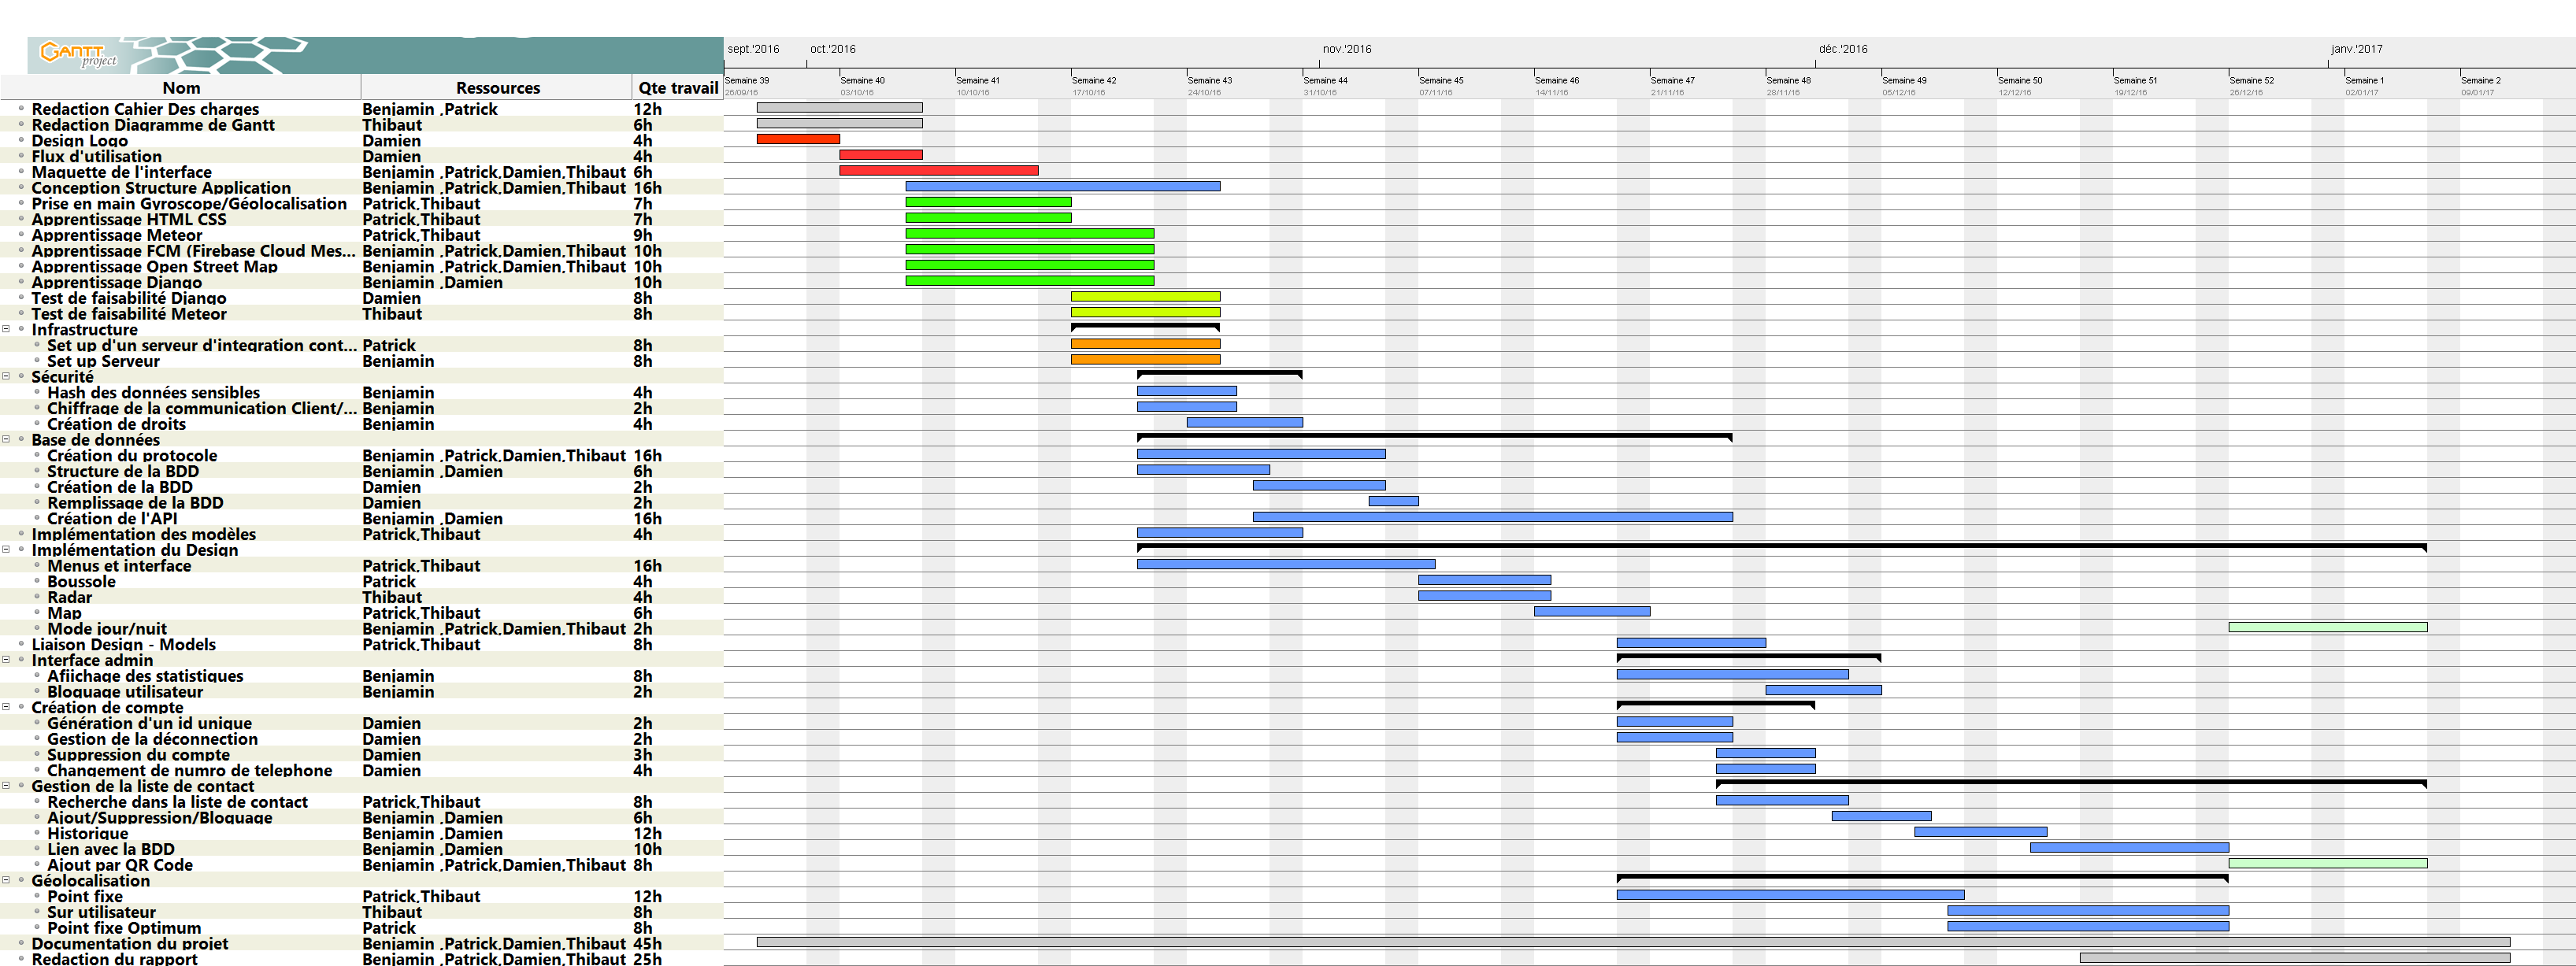
\includegraphics[angle=90,width=\linewidth,height=\textheight]{../diagramme-de-gantt/diagramme-de-gantt.png}
			\centering
			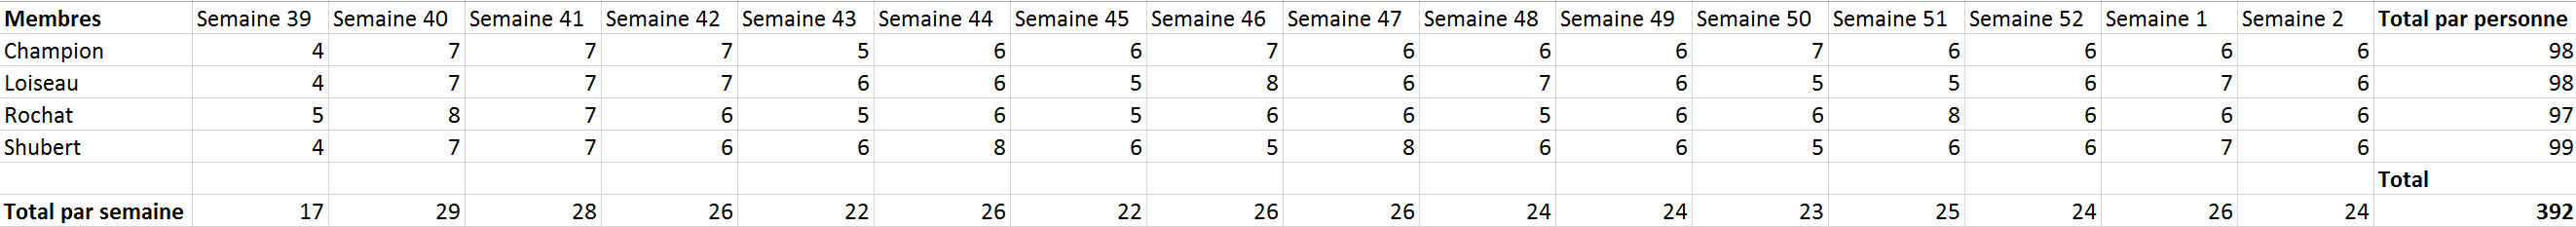
\includegraphics[angle=90,height=\textheight]{../diagramme-de-gantt/tableau-heures-personnes}
				

\end{document}
